\chapter{Feature Extraction}

总结文章:\href{https://zhuanlan.zhihu.com/p/35724768}{Object Detection总结 Two Stage}

总结文章:\href{https://zhuanlan.zhihu.com/p/35731743}{Object Detection总结 One Stage}

\section{Selective Search}

\subsection{Efficient Graph-Based Image Segmentation}

Selective Search基于文章\cite{Felzenszwalb2004}中基于图分割的图像分割技术。

论文\cite{Felzenszwalb2004}提出的是一种基于贪心选择的图像分割算法,论文中把图像中的每个像素表示图上的一个节点,每一条连接节点的无向边都具有一个权重(weights),以衡量其连接的两个节点之间的不相似度,这篇论文的创新点在于该算法能够根据相邻区域在特征值上变化速度的大小动态调整分割阈值。这个特征值就是类间距离和类内距离,如果类间距离大于类内距离就认为是两个区域。定义类内距离为对应区域的最小生成树(因为把图像看做一个连接图,所以每个区域可以用最小生成树来表示)中权重最大的边的权重值,类间距离定义为两个区域内相邻点的最小权重边,如果两个区域没有相邻边则取无穷大。但是这样其实还是有问题,比如一个类中只有一个点的时候,它的类内距离为0,这样就没法搞了(每个点都变成了一类,此时类内距离变为0),所以作者又引入了一个阈值函数,用来表示两个区域的区域的类间距离至少要比类内距离大多少才能认为是两个区域。

判断两个点$C_1$与$C_2$是否属于同一类的判定:
\begin{displaymath}
D(C_1, C_2) = 
\begin{cases}
true & \text{if } Dif(C_1, C_2) > M Int(C_1, C_2)\\
false & \text{otherwise}
\end{cases}
\end{displaymath}
其中,$MInt(C_1, C_2)$为判断类间间距$Dif$的阈值,由类内间距计算得到:
\begin{displaymath}
M Int(C_1, C_2) = \min (Int(C_1) + \tau (C_1), Int(C_2) + \tau (C_2) )
\end{displaymath}
其中,$\tau$即为控制当类间的最短距离。一般取为$C$的负相关函数,$k$为常数:
\[
\tau(C) = k / |C|
\]
当$k$的取值大时,类间距要求大,所以分割后的区域面积也会较大,否则区域面积较小。

具体的分割过程,可以参考文章\cite{Felzenszwalb2004}的\textbf{Algorithm 1}。

\subsection{Selective Search}
主要参考文献:\cite{Uijlings2013}

接下来介绍Selective Search算法,该算法利用\cite{Felzenszwalb2004}的图分割算法获得的分割区域结果,再一次根据一些搜索策略(相似度)做了一个聚类。也是和上面的思路一致,首先根据获得的区域,算出每个区域和其他区域的相似度,不相邻的和自身与自身的相似度都设置为0,得到一个N*N的矩阵,然后将相似度最大的合并,再次计算相似度矩阵(这里是增量更新,只需要计算新生成的区域和其他区域的相似度就可以了),这样合并一次较少一个区域,对于N个区域需要执行N-1次合并,最终得到一个区域。对于相似度的度量,作者主要选取了颜色和区域两大块,颜色作者比较了8种模型,最终选择了HSV,区域主要考量大小、纹理和吻合度(相交包含关系)这三个因素。





\section{Region CNN}

\subsection{概述}

\begin{figure}[!htbp]
\centering
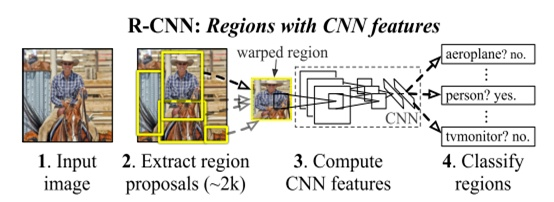
\includegraphics[width=0.85\textwidth]{FeatureExtraction/RCNN0.jpg}
\caption{RCNN整体思想}
\label{RCNN0}
\end{figure}

这里的 Extract region proposals 是基于Selective Search实现的,然后将这些候选框输入到CNN进行特征提取,最后利用SVM对提取的特征进行分类。







\section{SPP Net}


\section{Fast RCNN}

\section{Faster RCNN}

\section{R FCN}


\section{FPN}


\section{Mask RCNN}


\section{YOLO}


\section{YOLO v2}


\section{YOLO v3}


\section{SSD}


\section{DSSD}


\section{Retina Net (Focal Loss)}

